\documentclass[a4paper,12pt]{article}
\usepackage{float}
\usepackage[table]{xcolor} % Para colorir as linhas da tabela
\usepackage{array} % Para melhorar a formatação de tabelas
\usepackage[brazil]{babel}
\usepackage[utf8]{inputenc}
\usepackage{indentfirst}
\usepackage{amsmath}
\usepackage{multicol}
\usepackage{graphicx}
\usepackage{animate}
\usepackage{tabularx}
\usepackage[font=footnotesize, labelfont=bf, listformat=empty]{caption}
\usepackage{geometry}
\usepackage{listings}
\usepackage{lastpage}
\usepackage{subcaption}
\usepackage[skins,xparse,breakable]{tcolorbox}
\usepackage{longtable}
\usepackage{minted}
\usepackage{titlesec}
\usepackage{fancyhdr}
\usepackage{setspace}
\usepackage[colorlinks=true, allcolors=black]{hyperref}

% Configurações de margens e espaçamento
\geometry{a4paper, left=2.5cm, right=2.5cm, top=2.5cm, bottom=2cm}
\onehalfspacing

% Configurações de títulos
\titleformat{\section}{\normalfont\large\bfseries}{\thesection}{1em}{}
\titleformat{\subsection}{\normalfont\bfseries}{\thesubsection}{1em}{}
\titleformat{\subsubsection}{\normalfont\itshape}{\thesubsubsection}{1em}{}

% Configurações de listagens
\renewcommand{\listingscaption}{Código}
\newenvironment{code}{\captionsetup{type=listing}}{}

% Configurações de cores
\definecolor{LightSeaGreen}{rgb}{0.1255, 0.6980, 0.6667}
\definecolor{whitesmoke}{rgb}{0.96, 0.96, 0.96}
\definecolor{cinza}{RGB}{160, 160, 160}
\definecolor{cinza_claro}{RGB}{240, 240, 240} % Cinza claro

% Configurações do minted para VHDL
\setminted[VHDL]{
    fontsize=\footnotesize,
    style=emacs,
    linenos=true,
    breaklines=true,
    mathescape=true,
    bgcolor=cinza_claro,
    breakanywhere=true,
}

\newcommand{\hex}[1]{\textcolor{green!50!black}{#1}}

% Configurações de cabeçalho e rodapé
\pagestyle{fancy}
\fancyhf{}
\fancyhead[L]{\footnotesize{Laboratório de Sistemas Digitais - ENE0040}}
\fancyhead[R]{\footnotesize{2025/1 - Turma 07}}
\fancyfoot[R]{\footnotesize{Página \hspace{0.05cm} \thepage \hspace{0.05cm} de \pageref{LastPage}}}
\fancyfoot[L]{\footnotesize{Relatório do Experimento 6}}

% Adiciona uma linha preta acima do rodapé
\renewcommand{\footrulewidth}{0.4pt} % Espessura da linha
\renewcommand{\footrule}{\vbox to 0pt{\hrule width \textwidth height \footrulewidth \vss}} % Desenha a linha

% Novo Comando para chamar a capa
\newcommand{\capa}{
    \begin{titlepage}
        \begin{multicols}{2}
            \begin{flushleft}
                
\includegraphics[width=0.45\linewidth]{Recursos/Imagens/UnB_logo.png}
            \end{flushleft}
            \columnbreak
            \begin{flushright}
                Universidade de Brasília \\
                Faculdade de Tecnologia \\
                Departamento de Engenharia Elétrica
            \end{flushright}
        \end{multicols}
        \begin{center}
        \vspace{-20pt}
        \rule{\textwidth}{0.4pt}
        \end{center}
        \vspace{0.6cm}
        \begin{center}
            {\Huge \textbf{Relatório do Experimento 6}} \\[1em]
            {\large \textbf{Autor:} Henrique Morcelles Salum} \\[0.5em]
            {\large \textbf{Matrícula:} 232003008} \\
            \vfill
            {\large \textbf{ENE0040 - Laboratório de Sistemas Digitais - Turma 07}} \\
        \end{center}
    \end{titlepage}
}

\begin{document}

\capa

% Sumário
\newpage
\tableofcontents
\newpage

% Introdução
\section{Introdução}

\subsection{Sobre o Experimento}
Este experimento é composto por duas tarefas; em ambas, deve-se escrever códigos em VHDL que implementem sistemas digitais e simulá-los no \textit{software} ModelSim, da Intel.

\subsubsection{Flip-Flop JK}
Na primeira tarefa, devemos utilizar a estrutura ``process'' para implementar um flip-flop JK gatilhado pela borda de subida. A tabela-verdade desse sistema está apresentada a seguir:
\begin{table}[H]
    \centering
    \footnotesize
    \begin{tabular}{|c|c|c|c|c|c|}
        \hline
        \rowcolor{black}
        \multicolumn{5}{|c|}{\textbf{\textcolor{white}{Entradas}}} & \multicolumn{1}{|c|}{\textbf{\textcolor{white}{Saída}}} \\ \hline
        \rowcolor{black}
        \textcolor{white}{\textbf{PR}} & \textcolor{white}{\textbf{CLR}} & \textcolor{white}{\textbf{CLK}} & \textcolor{white}{\textbf{J}} & \textcolor{white}{\textbf{K}} & \textcolor{white}{\textbf{Q}} \\ \hline
        1 & $\mathsf{X}$ & $\mathsf{X}$ & $\mathsf{X}$ & $\mathsf{X}$ & 1 \\ \hline
        \rowcolor{cinza}
        0 & 1 & $\mathsf{X}$ & $\mathsf{X}$ & $\mathsf{X}$ & 0 \\ \hline
        0 & 0 & 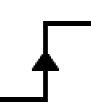
\includegraphics[width=0.02\linewidth]{Recursos/Imagens/subida_clock.png} & 0 & 0 & $LastQ$ \\ \hline
        \rowcolor{cinza}
        0 & 0 & 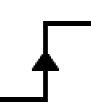
\includegraphics[width=0.02\linewidth]{Recursos/Imagens/subida_clock.png} & 0 & 1 & 0 \\ \hline
        0 & 0 & 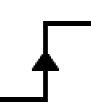
\includegraphics[width=0.02\linewidth]{Recursos/Imagens/subida_clock.png} & 1 & 0 & 1 \\ \hline
        \rowcolor{cinza}
        0 & 0 & 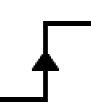
\includegraphics[width=0.02\linewidth]{Recursos/Imagens/subida_clock.png} & 1 & 1 & $\overline{LastQ}$\\ \hline
        0 & 0 & outros & $\mathsf{X}$ & $\mathsf{X}$ & $LastQ$\\ \hline
    \end{tabular}
    \caption{Tabela-verdade do flip-flop JK}
    \label{tab: q1_1}
\end{table}

\subsubsection{Registrador de Deslocamento}
A segunda tarefa consiste em implementar, novamente por meio da estrutura ``process'', um registrador de deslocamento bidirecional gatilhado pela borda de subida e dotado das entradas \textbf{RST} (\textit{reset}) e \textbf{LOAD}. Esse sistema é descrito pela tabela-verdade a seguir.

\begin{table}[H]
    \centering
    \footnotesize
    \begin{tabular}{|c|c|c|c|c|c|c|c|}
        \hline
        \rowcolor{black}
        \multicolumn{7}{|c|}{\textbf{\textcolor{white}{Entradas}}} & \textbf{\textcolor{white}{Saída}} \\ \hline
        \rowcolor{black}
        \textcolor{white}{\textbf{CLK}} & \textcolor{white}{\textbf{RST}} & \textcolor{white}{\textbf{LOAD}} & \textcolor{white}{\textbf{D}} & \textcolor{white}{\textbf{DIR}} & \textcolor{white}{\textbf{L}} & \textcolor{white}{\textbf{R}} & \textcolor{white}{\textbf{Q}} \\ \hline
        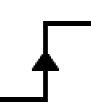
\includegraphics[width=0.02\linewidth]{Recursos/Imagens/subida_clock.png} & 1 & $\mathsf{X}$ & $\mathsf{X} \mathsf{X}  \mathsf{X}  \mathsf{X} $ & $\mathsf{X}$ & $\mathsf{X}$ & $\mathsf{X}$ & 0000 \\ \hline
        \rowcolor{cinza}
        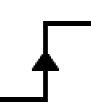
\includegraphics[width=0.02\linewidth]{Recursos/Imagens/subida_clock.png} & 0 & 1 & $D_3D_2D_1D_0$ & $\mathsf{X}$ & $\mathsf{X}$ & $\mathsf{X}$ & $D_3D_2D_1D_0$ \\ \hline
        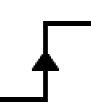
\includegraphics[width=0.02\linewidth]{Recursos/Imagens/subida_clock.png} & 0 & 0 & $\mathsf{X} \mathsf{X}  \mathsf{X}  \mathsf{X} $ & 0 & 0 & $\mathsf{X}$ & $Q_2Q_1Q_0$0 \\ \hline
        \rowcolor{cinza}
        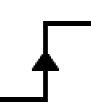
\includegraphics[width=0.02\linewidth]{Recursos/Imagens/subida_clock.png} & 0 & 0 & $\mathsf{X} \mathsf{X}  \mathsf{X}  \mathsf{X} $ & 0 & 1 & $\mathsf{X}$ & $Q_2Q_1Q_0$1 \\ \hline
        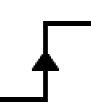
\includegraphics[width=0.02\linewidth]{Recursos/Imagens/subida_clock.png} & 0 & 0 & $\mathsf{X} \mathsf{X}  \mathsf{X}  \mathsf{X} $ & 1 & $\mathsf{X}$ & 0 & $0Q_3Q_2Q_1$ \\ \hline
        \rowcolor{cinza}
        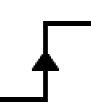
\includegraphics[width=0.02\linewidth]{Recursos/Imagens/subida_clock.png} & 0 & 0 & $\mathsf{X} \mathsf{X}  \mathsf{X}  \mathsf{X} $ & 1 & $\mathsf{X}$ & 1 & $1Q_3Q_2Q_1$ \\ \hline
        outros & $\mathsf{X}$ & $\mathsf{X}$ & $\mathsf{X} \mathsf{X}  \mathsf{X}  \mathsf{X} $ & $\mathsf{X}$ & $\mathsf{X}$ & $\mathsf{X}$ & $Q_3Q_2Q_1Q_0$ \\ \hline
    \end{tabular}
    \caption{Tabela-verdade do registrador de deslocamento}
    \label{tab:shift_register}
    \vspace{-5pt}
\end{table}

Para implementar esse registrador, além do código do flip-flop, que será apresentado doravante, foram utilizados multiplexadores 4x1. Isso não seria necessário de acordo com o roteiro, foi uma decisão minha (avalizada pelo professor) implementar o registrador em mais baixo nível (com uma arquitetura estrutural), o que exigiu o uso do multiplexador.

\subsection{Introdução Teórica}

\subsubsection{Flip-flops e Circuitos Sequenciais}
Os \textbf{flip-flops} são circuitos digitais fundamentais na eletrônica digital, responsáveis por armazenar informações binárias. Diferentemente das portas lógicas combinacionais, cuja saída depende unicamente das entradas atuais, os flip-flops fazem parte dos chamados circuitos sequenciais, nos quais a saída depende não apenas das entradas atuais, mas também do \textit{estado anterior} do sistema. Essa característica os torna essenciais na implementação de memórias, registradores, contadores, máquinas de estados finitos e diversos sistemas digitais temporizados.

\begin{figure}[H]
    \centering
    % Important: If latex complains about unicode characters,
% please use "\usepackage[utf8x]{inputenc}" in your preamble
% You can change the size of the picture by putting it into the construct:
% 1) \resizebox{10cm}{!}{"below picture"} to scale horizontally to 10 cm
% 2) \resizebox{!}{15cm}{"below picture"} to scale vertically to 15 cm
% 3) \resizebox{10cm}{15cm}{"below picture"} a combination of above two
% It is not recomended to use the scale option of the tikzpicture environment.
\begin{tikzpicture}[x=1pt,y=-1pt,line cap=rect]
\useasboundingbox (0,0) rectangle (125,100);
\def\logisimfontA#1{\fontfamily{cmr}{#1}} % Replaced by logisim, original font was "SansSerif"
\def\logisimfontB#1{\fontfamily{Ubuntu}{#1}}
\definecolor{custcol_0_0_0}{RGB}{0, 0, 0}
\definecolor{custcol_75_75_75}{RGB}{117, 117, 117}
\definecolor{custcol_ff_ff_ff}{RGB}{255, 255, 255}
\draw [line width=3.0pt, custcol_0_0_0 ]  (65.0,115.0) -- (65.0,125.0) ;
\draw [line width=3.0pt, custcol_0_0_0 ]  (5.0,95.0) -- (15.0,95.0) ;
\draw [line width=3.0pt, custcol_0_0_0 ]  (115.0,65.0) -- (125.0,65.0) ;
\draw [line width=3.0pt, custcol_0_0_0 ]  (5.0,35.0) -- (15.0,35.0) ;
\draw [line width=3.0pt, custcol_0_0_0 ]  (45.0,5.0) -- (45.0,15.0) ;
\draw [line width=3.0pt, custcol_0_0_0 ]  (85.0,5.0) -- (85.0,15.0) ;
\draw [line width=1.0pt, custcol_0_0_0 ]  (15.0,15.0) -- (114.0,15.0) ;
\draw [line width=1.0pt, custcol_0_0_0 ]  (115.0,15.0) -- (115.0,114.0) ;
\draw [line width=1.0pt, custcol_0_0_0 ]  (115.0,115.0) -- (16.0,115.0) ;
\draw [line width=1.0pt, custcol_0_0_0 ]  (15.0,115.0) -- (15.0,16.0) ;
\draw [line width=1.0pt, custcol_0_0_0 ]  (65.0,105.0) -- (63.0,115.0) -- (67.0,115.0) -- cycle;
\logisimfontB{\fontsize{16pt}{16pt}\fontseries{bx}\selectfont\node[inner sep=0, outer sep=0, custcol_0_0_0, anchor=base west] at  (23.0,40.0)  {J};}
\logisimfontB{\fontsize{16pt}{16pt}\fontseries{bx}\selectfont\node[inner sep=0, outer sep=0, custcol_0_0_0, anchor=base west] at  (22.0,100.0)  {K};}
\logisimfontB{\fontsize{16pt}{16pt}\fontseries{bx}\selectfont\node[inner sep=0, outer sep=0, custcol_0_0_0, anchor=base west] at  (94.0,69.0)  {Q};}
\logisimfontB{\fontsize{14pt}{14pt}\fontseries{bx}\selectfont\node[inner sep=0, outer sep=0, custcol_75_75_75, anchor=base west] at  (36.0,33.0)  {PR};}
\logisimfontB{\fontsize{14pt}{14pt}\fontseries{bx}\selectfont\node[inner sep=0, outer sep=0, custcol_75_75_75, anchor=base west] at  (73.0,33.0)  {CLR};}
\logisimfontB{\fontsize{14pt}{14pt}\fontseries{bx}\selectfont\node[inner sep=0, outer sep=0, custcol_75_75_75, anchor=base west] at  (52.0,101.0)  {CLK};}
\fill [line width=1.0pt, custcol_0_0_0]  (15.0,35.0) ellipse (2.0 and 2.0 );
\fill [line width=1.0pt, custcol_0_0_0]  (15.0,95.0) ellipse (2.0 and 2.0 );
\fill [line width=1.0pt, custcol_0_0_0]  (45.0,15.0) ellipse (2.0 and 2.0 );
\fill [line width=1.0pt, custcol_0_0_0]  (65.0,115.0) ellipse (2.0 and 2.0 );
\fill [line width=1.0pt, custcol_0_0_0]  (85.0,15.0) ellipse (2.0 and 2.0 );
\fill [line width=1.0pt, custcol_0_0_0]  (115.0,65.0) ellipse (2.0 and 2.0 );
\end{tikzpicture}


    \caption{Flip-flop JK}
    \label{fig:enter-label}
\end{figure}
Um flip-flop é capaz de armazenar um único bit de informação e muda de estado geralmente em função de um sinal de controle denominado \textbf{clock} (CLK). As transições ocorrem, nas bordas de subida (ou descida) desse sinal de clock, o que sincroniza a operação de múltiplos flip-flops em um sistema.

O comportamento do flip-flop JK, objeto desse experimento, está descrito na \autoref{tab: q1_1}. A operação da penúltima linha dessa tabela — de \textit{toggle} ou comutação — torna o flip-flop JK particularmente útil na construção de contadores binários, nos quais o estado se alterna a cada pulso de clock. Além disso, o comportamento bem definido para todos os pares de entradas diferencia o flip-flop JK do flip-flop RS, que apresenta uma condição inválida quando ambas as entradas são 1.

\subsubsection{Registradores}
Na eletrônica digital, um registrador é um circuito sequencial síncrono composto por um conjunto de flip-flops, geralmente do tipo D ou JK, que armazena um grupo de bits simultaneamente. Cada flip-flop representa uma posição de armazenamento de um bit, e, juntos, formam uma unidade capaz de armazenar palavras binárias de múltiplos bits. Os registradores são componentes essenciais em microprocessadores, microcontroladores e em diversas arquiteturas digitais, pois atuam como memória de curto prazo e mecanismos de transferência de dados.

Um tipo especial de registrador é o registrador de deslocamento (\textit{shift register}). Ele permite que os dados armazenados sejam deslocados, bit a bit, para a esquerda ou para a direita, em cada pulso de clock. Essa funcionalidade é útil para diversas aplicações. Tipicamente, processadores são dotados desses dispositivos; na programação em assembly, eles são diretamente manipulados pelo programador e, em linguagens de alto nível, a sua manipulação é abstraída por meio de variáveis.

\begin{figure}[H]
    \centering
    % Important: If latex complains about unicode characters,
% please use "\usepackage[utf8x]{inputenc}" in your preamble
% You can change the size of the picture by putting it into the construct:
% 1) \resizebox{10cm}{!}{"below picture"} to scale horizontally to 10 cm
% 2) \resizebox{!}{15cm}{"below picture"} to scale vertically to 15 cm
% 3) \resizebox{10cm}{15cm}{"below picture"} a combination of above two
% It is not recomended to use the scale option of the tikzpicture environment.
\scalebox{0.6}{
\begin{tikzpicture}[x=1pt,y=-1pt,line cap=rect]
\def\logisimfontA#1{\fontfamily{cmr}{#1}} % Replaced by logisim, original font was "SansSerif"
\def\logisimfontB#1{\fontfamily{Ubuntu}{#1}}
\def\logisimfontC#1{\fontfamily{cmtt}{#1}} % Replaced by logisim, original font was "Monospaced"
\definecolor{custcol_0_0_0}{RGB}{0, 0, 0}
\definecolor{custcol_75_75_75}{RGB}{117, 117, 117}
\definecolor{custcol_ff_ff_ff}{RGB}{255, 255, 255}
\draw [line width=3.0pt, custcol_0_0_0 ]  (349.0,538.0) -- (349.0,548.0) ;
\draw [line width=4.0pt, custcol_0_0_0 ]  (219.0,128.0) -- (219.0,148.0) ;
\draw [line width=3.0pt, custcol_0_0_0 ]  (149.0,58.0) -- (149.0,98.0) -- (199.0,98.0) ;
\draw [line width=3.0pt, custcol_0_0_0 ]  (19.0,58.0) -- (19.0,68.0) ;
\draw [line width=3.0pt, custcol_0_0_0 ]  (59.0,58.0) -- (59.0,68.0) ;
\draw [line width=3.0pt, custcol_0_0_0 ]  (349.0,348.0) -- (349.0,358.0) ;
\draw [line width=4.0pt, custcol_0_0_0 ]  (219.0,698.0) -- (219.0,718.0) ;
\draw [line width=3.0pt, custcol_0_0_0 ]  (329.0,608.0) -- (329.0,628.0) ;
\draw [line width=3.0pt, custcol_0_0_0 ]  (369.0,608.0) -- (369.0,628.0) ;
\draw [line width=4.0pt, custcol_0_0_0 ]  (99.0,58.0) -- (99.0,88.0) ;
\draw [line width=3.0pt, custcol_0_0_0 ]  (299.0,458.0) -- (259.0,458.0) -- (259.0,488.0) -- (259.0,518.0) -- (289.0,518.0) ;
\draw [line width=4.0pt, custcol_0_0_0 ]  (589.0,98.0) -- (609.0,98.0) ;
\draw [line width=3.0pt, custcol_0_0_0 ]  (229.0,488.0) -- (259.0,488.0) ;
\draw [line width=3.0pt, custcol_0_0_0 ]  (199.0,308.0) -- (169.0,308.0) -- (169.0,428.0) -- (429.0,428.0) -- (429.0,488.0) -- (399.0,488.0) ;
\draw [line width=3.0pt, custcol_0_0_0 ]  (349.0,158.0) -- (349.0,168.0) ;
\draw [line width=4.0pt, custcol_0_0_0 ]  (219.0,508.0) -- (219.0,528.0) ;
\draw [line width=3.0pt, custcol_0_0_0 ]  (329.0,418.0) -- (329.0,438.0) ;
\draw [line width=3.0pt, custcol_0_0_0 ]  (369.0,418.0) -- (369.0,438.0) ;
\draw [line width=3.0pt, custcol_0_0_0 ]  (299.0,268.0) -- (259.0,268.0) -- (259.0,298.0) -- (259.0,328.0) -- (289.0,328.0) ;
\draw [line width=3.0pt, custcol_0_0_0 ]  (169.0,238.0) -- (169.0,118.0) -- (199.0,118.0) ;
\draw [line width=3.0pt, custcol_0_0_0 ]  (229.0,298.0) -- (259.0,298.0) ;
\draw [line width=3.0pt, custcol_0_0_0 ]  (399.0,108.0) -- (429.0,108.0) -- (479.0,108.0) -- (479.0,198.0) -- (159.0,198.0) -- (159.0,288.0) -- (199.0,288.0) ;
\draw [line width=3.0pt, custcol_0_0_0 ]  (199.0,278.0) -- (169.0,278.0) -- (169.0,238.0) -- (429.0,238.0) -- (429.0,298.0) ;
\draw [line width=3.0pt, custcol_0_0_0 ]  (199.0,478.0) -- (159.0,478.0) -- (159.0,388.0) -- (479.0,388.0) -- (479.0,298.0) -- (429.0,298.0) -- (399.0,298.0) ;
\draw [line width=3.0pt, custcol_0_0_0 ]  (349.0,728.0) -- (349.0,738.0) ;
\draw [line width=4.0pt, custcol_0_0_0 ]  (219.0,318.0) -- (219.0,338.0) ;
\draw [line width=3.0pt, custcol_0_0_0 ]  (329.0,228.0) -- (329.0,248.0) ;
\draw [line width=3.0pt, custcol_0_0_0 ]  (369.0,228.0) -- (369.0,248.0) ;
\draw [line width=3.0pt, custcol_0_0_0 ]  (259.0,678.0) -- (259.0,708.0) -- (289.0,708.0) ;
\draw [line width=3.0pt, custcol_0_0_0 ]  (329.0,28.0) -- (329.0,58.0) ;
\draw [line width=3.0pt, custcol_0_0_0 ]  (369.0,28.0) -- (369.0,58.0) ;
\draw [line width=3.0pt, custcol_0_0_0 ]  (479.0,488.0) -- (479.0,578.0) -- (159.0,578.0) -- (159.0,668.0) -- (199.0,668.0) ;
\draw [line width=3.0pt, custcol_0_0_0 ]  (229.0,678.0) -- (259.0,678.0) -- (259.0,648.0) -- (299.0,648.0) ;
\draw [line width=3.0pt, custcol_0_0_0 ]  (229.0,108.0) -- (259.0,108.0) ;
\draw [line width=3.0pt, custcol_0_0_0 ]  (299.0,78.0) -- (259.0,78.0) -- (259.0,108.0) -- (259.0,138.0) -- (289.0,138.0) ;
\draw [line width=3.0pt, custcol_0_0_0 ]  (399.0,678.0) -- (429.0,678.0) ;
\draw [line width=3.0pt, custcol_0_0_0 ]  (169.0,428.0) -- (169.0,468.0) -- (199.0,468.0) ;
\draw [line width=3.0pt, custcol_0_0_0 ]  (199.0,88.0) -- (169.0,88.0) -- (169.0,48.0) -- (429.0,48.0) -- (429.0,108.0) ;
\draw [line width=3.0pt, custcol_0_0_0 ]  (129.0,58.0) -- (129.0,688.0) -- (199.0,688.0) ;
\draw [line width=3.0pt, custcol_0_0_0 ]  (199.0,498.0) -- (169.0,498.0) -- (169.0,618.0) ;
\fill [line width=3.0pt, custcol_0_0_0]  (429.0,298.0) ellipse (5.0 and 5.0 );
\fill [line width=3.0pt, custcol_0_0_0]  (169.0,428.0) ellipse (5.0 and 5.0 );
\fill [line width=3.0pt, custcol_0_0_0]  (479.0,298.0) ellipse (5.0 and 5.0 );
\fill [line width=3.0pt, custcol_0_0_0]  (259.0,488.0) ellipse (5.0 and 5.0 );
\fill [line width=3.0pt, custcol_0_0_0]  (429.0,108.0) ellipse (5.0 and 5.0 );
\fill [line width=3.0pt, custcol_0_0_0]  (169.0,238.0) ellipse (5.0 and 5.0 );
\fill [line width=3.0pt, custcol_0_0_0]  (479.0,108.0) ellipse (5.0 and 5.0 );
\fill [line width=3.0pt, custcol_0_0_0]  (259.0,298.0) ellipse (5.0 and 5.0 );
\fill [line width=3.0pt, custcol_0_0_0]  (429.0,678.0) ellipse (5.0 and 5.0 );
\fill [line width=3.0pt, custcol_0_0_0]  (259.0,108.0) ellipse (5.0 and 5.0 );
\fill [line width=3.0pt, custcol_0_0_0]  (429.0,488.0) ellipse (5.0 and 5.0 );
\fill [line width=3.0pt, custcol_0_0_0]  (169.0,618.0) ellipse (5.0 and 5.0 );
\fill [line width=3.0pt, custcol_0_0_0]  (479.0,488.0) ellipse (5.0 and 5.0 );
\fill [line width=3.0pt, custcol_0_0_0]  (259.0,678.0) ellipse (5.0 and 5.0 );
\draw [line width=2.0pt, custcol_0_0_0 ]  (9.0,38.0) -- (28.0,38.0) ;
\draw [line width=2.0pt, custcol_0_0_0 ]  (29.0,38.0) -- (29.0,57.0) ;
\draw [line width=2.0pt, custcol_0_0_0 ]  (29.0,58.0) -- (10.0,58.0) ;
\draw [line width=2.0pt, custcol_0_0_0 ]  (9.0,58.0) -- (9.0,39.0) ;
\draw [line width=2.0pt, custcol_0_0_0 ]  (13.0,48.0) -- (13.0,44.0) -- (19.0,44.0) -- (19.0,52.0) -- (25.0,52.0) -- (25.0,48.0) ;
\fill [line width=2.0pt, custcol_0_0_0]  (19.0,58.0) ellipse (2.0 and 2.0 );
\logisimfontB{\fontsize{12pt}{12pt}\fontseries{bx}\selectfont\node[inner sep=0, outer sep=0, custcol_0_0_0, anchor=base west] at  (9.0,85.0)  {CLK};}
\draw [line width=2.0pt, custcol_0_0_0 ]  (6.0,72.0) -- (9.0,72.0) -- (19.0,68.0) -- (29.0,72.0) -- (33.0,72.0) -- (33.0,91.0) -- (6.0,91.0) -- cycle;
\fill [line width=2.0pt, custcol_0_0_0]  (19.0,68.0) ellipse (2.0 and 2.0 );
\draw [line width=2.0pt, custcol_0_0_0 ]  (51.0,40.0) -- (68.0,40.0) ;
\draw [line width=2.0pt, custcol_0_0_0 ]  (69.0,40.0) -- (69.0,57.0) ;
\draw [line width=2.0pt, custcol_0_0_0 ]  (69.0,58.0) -- (52.0,58.0) ;
\draw [line width=2.0pt, custcol_0_0_0 ]  (51.0,58.0) -- (51.0,41.0) ;
\logisimfontA{\fontsize{12pt}{12pt}\selectfont\node[inner sep=0, outer sep=0, custcol_0_0_0, anchor=base west] at  (53.0,55.0)  {x1};}
\logisimfontB{\fontsize{16pt}{16pt}\fontseries{bx}\selectfont\node[inner sep=0, outer sep=0, custcol_0_0_0, anchor=base west] at  (45.0,33.0)  {RST};}
\fill [line width=2.0pt, custcol_0_0_0]  (59.0,58.0) ellipse (2.0 and 2.0 );
\logisimfontB{\fontsize{12pt}{12pt}\fontseries{bx}\selectfont\node[inner sep=0, outer sep=0, custcol_0_0_0, anchor=base west] at  (49.0,85.0)  {RST};}
\draw [line width=2.0pt, custcol_0_0_0 ]  (46.0,72.0) -- (49.0,72.0) -- (59.0,68.0) -- (69.0,72.0) -- (73.0,72.0) -- (73.0,91.0) -- (46.0,91.0) -- cycle;
\fill [line width=2.0pt, custcol_0_0_0]  (59.0,68.0) ellipse (2.0 and 2.0 );
\draw [line width=3.0pt, custcol_0_0_0 ]  (199.0,128.0) -- (109.0,128.0) -- (109.0,108.0) -- (109.0,94.0) ;
\draw [line width=3.0pt, custcol_0_0_0 ]  (199.0,318.0) -- (99.0,318.0) -- (99.0,108.0) -- (99.0,94.0) ;
\draw [line width=3.0pt, custcol_0_0_0 ]  (199.0,508.0) -- (89.0,508.0) -- (89.0,108.0) -- (89.0,94.0) ;
\draw [line width=3.0pt, custcol_0_0_0 ]  (199.0,698.0) -- (79.0,698.0) -- (79.0,108.0) -- (79.0,94.0) ;
\draw [line width=5.0pt, custcol_0_0_0 ]  (99.0,89.0) -- (99.0,94.0) ;
\draw [line width=5.0pt, custcol_0_0_0 ]  (108.0,94.0) -- (80.0,94.0) ;
\logisimfontA{\fontsize{7pt}{7pt}\selectfont\node[inner sep=0, outer sep=0, custcol_0_0_0, anchor=base west, rotate=-90.0] at  (112.0,97.0)  {3};}
\logisimfontA{\fontsize{7pt}{7pt}\selectfont\node[inner sep=0, outer sep=0, custcol_0_0_0, anchor=base west, rotate=-90.0] at  (102.0,97.0)  {2};}
\logisimfontA{\fontsize{7pt}{7pt}\selectfont\node[inner sep=0, outer sep=0, custcol_0_0_0, anchor=base west, rotate=-90.0] at  (92.0,97.0)  {1};}
\logisimfontA{\fontsize{7pt}{7pt}\selectfont\node[inner sep=0, outer sep=0, custcol_0_0_0, anchor=base west, rotate=-90.0] at  (82.0,97.0)  {0};}
\fill [line width=5.0pt, custcol_0_0_0]  (99.0,88.0) ellipse (2.0 and 2.0 );
\fill [line width=5.0pt, custcol_0_0_0]  (109.0,108.0) ellipse (2.0 and 2.0 );
\fill [line width=5.0pt, custcol_0_0_0]  (99.0,108.0) ellipse (2.0 and 2.0 );
\fill [line width=5.0pt, custcol_0_0_0]  (89.0,108.0) ellipse (2.0 and 2.0 );
\fill [line width=5.0pt, custcol_0_0_0]  (79.0,108.0) ellipse (2.0 and 2.0 );
\draw [line width=2.0pt, custcol_0_0_0 ]  (81.0,40.0) -- (118.0,40.0) ;
\draw [line width=2.0pt, custcol_0_0_0 ]  (119.0,40.0) -- (119.0,57.0) ;
\draw [line width=2.0pt, custcol_0_0_0 ]  (119.0,58.0) -- (82.0,58.0) ;
\draw [line width=2.0pt, custcol_0_0_0 ]  (81.0,58.0) -- (81.0,41.0) ;
\logisimfontA{\fontsize{12pt}{12pt}\selectfont\node[inner sep=0, outer sep=0, custcol_0_0_0, anchor=base west] at  (93.0,55.0)  {x4};}
\logisimfontB{\fontsize{16pt}{16pt}\fontseries{bx}\selectfont\node[inner sep=0, outer sep=0, custcol_0_0_0, anchor=base west] at  (93.0,33.0)  {D};}
\fill [line width=2.0pt, custcol_0_0_0]  (99.0,58.0) ellipse (2.0 and 2.0 );
\draw [line width=2.0pt, custcol_0_0_0 ]  (121.0,40.0) -- (138.0,40.0) ;
\draw [line width=2.0pt, custcol_0_0_0 ]  (139.0,40.0) -- (139.0,57.0) ;
\draw [line width=2.0pt, custcol_0_0_0 ]  (139.0,58.0) -- (122.0,58.0) ;
\draw [line width=2.0pt, custcol_0_0_0 ]  (121.0,58.0) -- (121.0,41.0) ;
\logisimfontA{\fontsize{12pt}{12pt}\selectfont\node[inner sep=0, outer sep=0, custcol_0_0_0, anchor=base west] at  (123.0,55.0)  {x1};}
\logisimfontB{\fontsize{16pt}{16pt}\fontseries{bx}\selectfont\node[inner sep=0, outer sep=0, custcol_0_0_0, anchor=base west] at  (125.0,33.0)  {L};}
\fill [line width=2.0pt, custcol_0_0_0]  (129.0,58.0) ellipse (2.0 and 2.0 );
\draw [line width=2.0pt, custcol_0_0_0 ]  (141.0,40.0) -- (158.0,40.0) ;
\draw [line width=2.0pt, custcol_0_0_0 ]  (159.0,40.0) -- (159.0,57.0) ;
\draw [line width=2.0pt, custcol_0_0_0 ]  (159.0,58.0) -- (142.0,58.0) ;
\draw [line width=2.0pt, custcol_0_0_0 ]  (141.0,58.0) -- (141.0,41.0) ;
\logisimfontA{\fontsize{12pt}{12pt}\selectfont\node[inner sep=0, outer sep=0, custcol_0_0_0, anchor=base west] at  (143.0,55.0)  {x1};}
\logisimfontA{\fontsize{16pt}{16pt}\fontseries{bx}\selectfont\node[inner sep=0, outer sep=0, custcol_0_0_0, anchor=base west] at  (144.0,31.0)  {R};}
\fill [line width=2.0pt, custcol_0_0_0]  (149.0,58.0) ellipse (2.0 and 2.0 );
\logisimfontB{\fontsize{16pt}{16pt}\fontseries{bx}\selectfont\node[inner sep=0, outer sep=0, custcol_0_0_0, anchor=base west] at  (215.0,167.0)  {S};}
\draw [line width=2.0pt, custcol_0_0_0 ]  (211.0,152.0) -- (219.0,148.0) -- (227.0,152.0) -- (227.0,174.0) -- (211.0,174.0) -- cycle;
\fill [line width=2.0pt, custcol_0_0_0]  (219.0,148.0) ellipse (2.0 and 2.0 );
\logisimfontB{\fontsize{16pt}{16pt}\fontseries{bx}\selectfont\node[inner sep=0, outer sep=0, custcol_0_0_0, anchor=base west] at  (215.0,357.0)  {S};}
\draw [line width=2.0pt, custcol_0_0_0 ]  (211.0,342.0) -- (219.0,338.0) -- (227.0,342.0) -- (227.0,364.0) -- (211.0,364.0) -- cycle;
\fill [line width=2.0pt, custcol_0_0_0]  (219.0,338.0) ellipse (2.0 and 2.0 );
\logisimfontB{\fontsize{16pt}{16pt}\fontseries{bx}\selectfont\node[inner sep=0, outer sep=0, custcol_0_0_0, anchor=base west] at  (215.0,547.0)  {S};}
\draw [line width=2.0pt, custcol_0_0_0 ]  (211.0,532.0) -- (219.0,528.0) -- (227.0,532.0) -- (227.0,554.0) -- (211.0,554.0) -- cycle;
\fill [line width=2.0pt, custcol_0_0_0]  (219.0,528.0) ellipse (2.0 and 2.0 );
\logisimfontB{\fontsize{16pt}{16pt}\fontseries{bx}\selectfont\node[inner sep=0, outer sep=0, custcol_0_0_0, anchor=base west] at  (215.0,737.0)  {S};}
\draw [line width=2.0pt, custcol_0_0_0 ]  (211.0,722.0) -- (219.0,718.0) -- (227.0,722.0) -- (227.0,744.0) -- (211.0,744.0) -- cycle;
\fill [line width=2.0pt, custcol_0_0_0]  (219.0,718.0) ellipse (2.0 and 2.0 );
\logisimfontC{\fontsize{12pt}{12pt}\selectfont\node[inner sep=0, outer sep=0, custcol_0_0_0, anchor=base west] at  (326.0,224.0)  {0};}
\fill [line width=1.0pt, custcol_0_0_0]  (329.0,228.0) ellipse (2.0 and 2.0 );
\logisimfontC{\fontsize{12pt}{12pt}\selectfont\node[inner sep=0, outer sep=0, custcol_0_0_0, anchor=base west] at  (326.0,414.0)  {0};}
\fill [line width=1.0pt, custcol_0_0_0]  (329.0,418.0) ellipse (2.0 and 2.0 );
\logisimfontC{\fontsize{12pt}{12pt}\selectfont\node[inner sep=0, outer sep=0, custcol_0_0_0, anchor=base west] at  (326.0,24.0)  {0};}
\fill [line width=1.0pt, custcol_0_0_0]  (329.0,28.0) ellipse (2.0 and 2.0 );
\logisimfontC{\fontsize{12pt}{12pt}\selectfont\node[inner sep=0, outer sep=0, custcol_0_0_0, anchor=base west] at  (326.0,604.0)  {0};}
\fill [line width=1.0pt, custcol_0_0_0]  (329.0,608.0) ellipse (2.0 and 2.0 );
\logisimfontB{\fontsize{12pt}{12pt}\fontseries{bx}\selectfont\node[inner sep=0, outer sep=0, custcol_0_0_0, anchor=base west] at  (339.0,185.0)  {CLK};}
\draw [line width=2.0pt, custcol_0_0_0 ]  (336.0,172.0) -- (339.0,172.0) -- (349.0,168.0) -- (359.0,172.0) -- (363.0,172.0) -- (363.0,191.0) -- (336.0,191.0) -- cycle;
\fill [line width=2.0pt, custcol_0_0_0]  (349.0,168.0) ellipse (2.0 and 2.0 );
\logisimfontB{\fontsize{12pt}{12pt}\fontseries{bx}\selectfont\node[inner sep=0, outer sep=0, custcol_0_0_0, anchor=base west] at  (339.0,375.0)  {CLK};}
\draw [line width=2.0pt, custcol_0_0_0 ]  (336.0,362.0) -- (339.0,362.0) -- (349.0,358.0) -- (359.0,362.0) -- (363.0,362.0) -- (363.0,381.0) -- (336.0,381.0) -- cycle;
\fill [line width=2.0pt, custcol_0_0_0]  (349.0,358.0) ellipse (2.0 and 2.0 );
\logisimfontB{\fontsize{12pt}{12pt}\fontseries{bx}\selectfont\node[inner sep=0, outer sep=0, custcol_0_0_0, anchor=base west] at  (339.0,565.0)  {CLK};}
\draw [line width=2.0pt, custcol_0_0_0 ]  (336.0,552.0) -- (339.0,552.0) -- (349.0,548.0) -- (359.0,552.0) -- (363.0,552.0) -- (363.0,571.0) -- (336.0,571.0) -- cycle;
\fill [line width=2.0pt, custcol_0_0_0]  (349.0,548.0) ellipse (2.0 and 2.0 );
\logisimfontB{\fontsize{12pt}{12pt}\fontseries{bx}\selectfont\node[inner sep=0, outer sep=0, custcol_0_0_0, anchor=base west] at  (339.0,755.0)  {CLK};}
\draw [line width=2.0pt, custcol_0_0_0 ]  (336.0,742.0) -- (339.0,742.0) -- (349.0,738.0) -- (359.0,742.0) -- (363.0,742.0) -- (363.0,761.0) -- (336.0,761.0) -- cycle;
\fill [line width=2.0pt, custcol_0_0_0]  (349.0,738.0) ellipse (2.0 and 2.0 );
\logisimfontB{\fontsize{12pt}{12pt}\fontseries{bx}\selectfont\node[inner sep=0, outer sep=0, custcol_0_0_0, anchor=base west] at  (359.0,220.0)  {RST};}
\draw [line width=2.0pt, custcol_0_0_0 ]  (356.0,205.0) -- (383.0,205.0) -- (383.0,225.0) -- (379.0,225.0) -- (369.0,229.0) -- (359.0,225.0) -- (356.0,225.0) -- cycle;
\fill [line width=2.0pt, custcol_0_0_0]  (369.0,228.0) ellipse (2.0 and 2.0 );
\logisimfontB{\fontsize{12pt}{12pt}\fontseries{bx}\selectfont\node[inner sep=0, outer sep=0, custcol_0_0_0, anchor=base west] at  (359.0,410.0)  {RST};}
\draw [line width=2.0pt, custcol_0_0_0 ]  (356.0,395.0) -- (383.0,395.0) -- (383.0,415.0) -- (379.0,415.0) -- (369.0,419.0) -- (359.0,415.0) -- (356.0,415.0) -- cycle;
\fill [line width=2.0pt, custcol_0_0_0]  (369.0,418.0) ellipse (2.0 and 2.0 );
\logisimfontB{\fontsize{12pt}{12pt}\fontseries{bx}\selectfont\node[inner sep=0, outer sep=0, custcol_0_0_0, anchor=base west] at  (359.0,20.0)  {RST};}
\draw [line width=2.0pt, custcol_0_0_0 ]  (356.0,5.0) -- (383.0,5.0) -- (383.0,25.0) -- (379.0,25.0) -- (369.0,29.0) -- (359.0,25.0) -- (356.0,25.0) -- cycle;
\fill [line width=2.0pt, custcol_0_0_0]  (369.0,28.0) ellipse (2.0 and 2.0 );
\logisimfontB{\fontsize{12pt}{12pt}\fontseries{bx}\selectfont\node[inner sep=0, outer sep=0, custcol_0_0_0, anchor=base west] at  (359.0,600.0)  {RST};}
\draw [line width=2.0pt, custcol_0_0_0 ]  (356.0,585.0) -- (383.0,585.0) -- (383.0,605.0) -- (379.0,605.0) -- (369.0,609.0) -- (359.0,605.0) -- (356.0,605.0) -- cycle;
\fill [line width=2.0pt, custcol_0_0_0]  (369.0,608.0) ellipse (2.0 and 2.0 );
\draw [line width=3.0pt, custcol_0_0_0 ]  (479.0,108.0) -- (569.0,108.0) -- (583.0,108.0) ;
\draw [line width=3.0pt, custcol_0_0_0 ]  (479.0,298.0) -- (509.0,298.0) -- (509.0,118.0) -- (569.0,118.0) -- (583.0,118.0) ;
\draw [line width=3.0pt, custcol_0_0_0 ]  (429.0,488.0) -- (479.0,488.0) -- (539.0,488.0) -- (539.0,128.0) -- (569.0,128.0) -- (583.0,128.0) ;
\draw [line width=3.0pt, custcol_0_0_0 ]  (199.0,658.0) -- (169.0,658.0) -- (169.0,618.0) -- (429.0,618.0) -- (429.0,678.0) -- (569.0,678.0) -- (569.0,138.0) -- (583.0,138.0) ;
\draw [line width=5.0pt, custcol_0_0_0 ]  (583.0,137.0) -- (583.0,104.0) -- (588.0,99.0) ;
\logisimfontA{\fontsize{7pt}{7pt}\selectfont\node[inner sep=0, outer sep=0, custcol_0_0_0, anchor=base west] at  (576.0,105.0)  {3};}
\logisimfontA{\fontsize{7pt}{7pt}\selectfont\node[inner sep=0, outer sep=0, custcol_0_0_0, anchor=base west] at  (576.0,115.0)  {2};}
\logisimfontA{\fontsize{7pt}{7pt}\selectfont\node[inner sep=0, outer sep=0, custcol_0_0_0, anchor=base west] at  (576.0,125.0)  {1};}
\logisimfontA{\fontsize{7pt}{7pt}\selectfont\node[inner sep=0, outer sep=0, custcol_0_0_0, anchor=base west] at  (576.0,135.0)  {0};}
\fill [line width=5.0pt, custcol_0_0_0]  (589.0,98.0) ellipse (2.0 and 2.0 );
\fill [line width=5.0pt, custcol_0_0_0]  (569.0,108.0) ellipse (2.0 and 2.0 );
\fill [line width=5.0pt, custcol_0_0_0]  (569.0,118.0) ellipse (2.0 and 2.0 );
\fill [line width=5.0pt, custcol_0_0_0]  (569.0,128.0) ellipse (2.0 and 2.0 );
\fill [line width=5.0pt, custcol_0_0_0]  (569.0,138.0) ellipse (2.0 and 2.0 );
\begin{pgfpicture}
   \begin{pgfmagnify}{1pt}{-1pt}
      \pgfsetrectcap
      \pgfsetcornersarced{\pgfpoint{3.0}{3.0}}
      \pgfsetlinewidth{2.0}
      \color{custcol_0_0_0}
      \pgfsetfillopacity{1.0}
      \pgfpathrectanglecorners{\pgfpoint{611.0}{90.0}}{\pgfpoint{649.0}{108.0}}
      \pgfusepath{stroke}
   \end{pgfmagnify}
\end{pgfpicture}
\logisimfontA{\fontsize{12pt}{12pt}\selectfont\node[inner sep=0, outer sep=0, custcol_0_0_0, anchor=base west] at  (623.0,105.0)  {x4};}
\logisimfontB{\fontsize{16pt}{16pt}\fontseries{bx}\selectfont\node[inner sep=0, outer sep=0, custcol_0_0_0, anchor=base west] at  (651.0,105.0)  {Q};}
\fill [line width=2.0pt, custcol_0_0_0]  (609.0,98.0) ellipse (2.0 and 2.0 );
\draw [line width=4.0pt, custcol_0_0_0 ]  (199.0,73.0) -- (199.0,143.0) -- (229.0,123.0) -- (229.0,93.0) -- cycle;
\fill [line width=1.0pt, custcol_0_0_0]  (199.0,88.0) ellipse (2.0 and 2.0 );
\fill [line width=1.0pt, custcol_0_0_0]  (199.0,98.0) ellipse (2.0 and 2.0 );
\fill [line width=1.0pt, custcol_0_0_0]  (199.0,118.0) ellipse (2.0 and 2.0 );
\fill [line width=1.0pt, custcol_0_0_0]  (199.0,128.0) ellipse (2.0 and 2.0 );
\fill [line width=1.0pt, custcol_0_0_0]  (219.0,128.0) ellipse (2.0 and 2.0 );
\fill [line width=1.0pt, custcol_0_0_0]  (229.0,108.0) ellipse (2.0 and 2.0 );
\draw [line width=4.0pt, custcol_0_0_0 ]  (199.0,263.0) -- (199.0,333.0) -- (229.0,313.0) -- (229.0,283.0) -- cycle;
\fill [line width=1.0pt, custcol_0_0_0]  (199.0,278.0) ellipse (2.0 and 2.0 );
\fill [line width=1.0pt, custcol_0_0_0]  (199.0,288.0) ellipse (2.0 and 2.0 );
\fill [line width=1.0pt, custcol_0_0_0]  (199.0,308.0) ellipse (2.0 and 2.0 );
\fill [line width=1.0pt, custcol_0_0_0]  (199.0,318.0) ellipse (2.0 and 2.0 );
\fill [line width=1.0pt, custcol_0_0_0]  (219.0,318.0) ellipse (2.0 and 2.0 );
\fill [line width=1.0pt, custcol_0_0_0]  (229.0,298.0) ellipse (2.0 and 2.0 );
\draw [line width=4.0pt, custcol_0_0_0 ]  (199.0,453.0) -- (199.0,523.0) -- (229.0,503.0) -- (229.0,473.0) -- cycle;
\fill [line width=1.0pt, custcol_0_0_0]  (199.0,468.0) ellipse (2.0 and 2.0 );
\fill [line width=1.0pt, custcol_0_0_0]  (199.0,478.0) ellipse (2.0 and 2.0 );
\fill [line width=1.0pt, custcol_0_0_0]  (199.0,498.0) ellipse (2.0 and 2.0 );
\fill [line width=1.0pt, custcol_0_0_0]  (199.0,508.0) ellipse (2.0 and 2.0 );
\fill [line width=1.0pt, custcol_0_0_0]  (219.0,508.0) ellipse (2.0 and 2.0 );
\fill [line width=1.0pt, custcol_0_0_0]  (229.0,488.0) ellipse (2.0 and 2.0 );
\draw [line width=4.0pt, custcol_0_0_0 ]  (199.0,643.0) -- (199.0,713.0) -- (229.0,693.0) -- (229.0,663.0) -- cycle;
\fill [line width=1.0pt, custcol_0_0_0]  (199.0,658.0) ellipse (2.0 and 2.0 );
\fill [line width=1.0pt, custcol_0_0_0]  (199.0,668.0) ellipse (2.0 and 2.0 );
\fill [line width=1.0pt, custcol_0_0_0]  (199.0,688.0) ellipse (2.0 and 2.0 );
\fill [line width=1.0pt, custcol_0_0_0]  (199.0,698.0) ellipse (2.0 and 2.0 );
\fill [line width=1.0pt, custcol_0_0_0]  (219.0,698.0) ellipse (2.0 and 2.0 );
\fill [line width=1.0pt, custcol_0_0_0]  (229.0,678.0) ellipse (2.0 and 2.0 );
\draw [line width=1.0pt, custcol_0_0_0 ]  (299.0,58.0) -- (398.0,58.0) ;
\draw [line width=1.0pt, custcol_0_0_0 ]  (399.0,58.0) -- (399.0,157.0) ;
\draw [line width=1.0pt, custcol_0_0_0 ]  (399.0,158.0) -- (300.0,158.0) ;
\draw [line width=1.0pt, custcol_0_0_0 ]  (299.0,158.0) -- (299.0,59.0) ;
\draw [line width=1.0pt, custcol_0_0_0 ]  (349.0,148.0) -- (347.0,158.0) -- (351.0,158.0) -- cycle;
\logisimfontB{\fontsize{16pt}{16pt}\fontseries{bx}\selectfont\node[inner sep=0, outer sep=0, custcol_0_0_0, anchor=base west] at  (307.0,83.0)  {J};}
\logisimfontB{\fontsize{16pt}{16pt}\fontseries{bx}\selectfont\node[inner sep=0, outer sep=0, custcol_0_0_0, anchor=base west] at  (306.0,143.0)  {K};}
\logisimfontB{\fontsize{16pt}{16pt}\fontseries{bx}\selectfont\node[inner sep=0, outer sep=0, custcol_0_0_0, anchor=base west] at  (378.0,112.0)  {Q};}
\logisimfontB{\fontsize{14pt}{14pt}\fontseries{bx}\selectfont\node[inner sep=0, outer sep=0, custcol_75_75_75, anchor=base west] at  (320.0,76.0)  {PR};}
\logisimfontB{\fontsize{14pt}{14pt}\fontseries{bx}\selectfont\node[inner sep=0, outer sep=0, custcol_75_75_75, anchor=base west] at  (357.0,76.0)  {CLR};}
\draw [line width=1.0pt, custcol_0_0_0]  (293.0,138.0) ellipse (5.0 and 5.0 );
\fill [line width=1.0pt, custcol_0_0_0]  (289.0,138.0) ellipse (2.0 and 2.0 );
\fill [line width=1.0pt, custcol_0_0_0]  (299.0,78.0) ellipse (2.0 and 2.0 );
\fill [line width=1.0pt, custcol_0_0_0]  (329.0,58.0) ellipse (2.0 and 2.0 );
\fill [line width=1.0pt, custcol_0_0_0]  (349.0,158.0) ellipse (2.0 and 2.0 );
\fill [line width=1.0pt, custcol_0_0_0]  (369.0,58.0) ellipse (2.0 and 2.0 );
\fill [line width=1.0pt, custcol_0_0_0]  (399.0,108.0) ellipse (2.0 and 2.0 );
\draw [line width=1.0pt, custcol_0_0_0 ]  (299.0,248.0) -- (398.0,248.0) ;
\draw [line width=1.0pt, custcol_0_0_0 ]  (399.0,248.0) -- (399.0,347.0) ;
\draw [line width=1.0pt, custcol_0_0_0 ]  (399.0,348.0) -- (300.0,348.0) ;
\draw [line width=1.0pt, custcol_0_0_0 ]  (299.0,348.0) -- (299.0,249.0) ;
\draw [line width=1.0pt, custcol_0_0_0 ]  (349.0,338.0) -- (347.0,348.0) -- (351.0,348.0) -- cycle;
\logisimfontB{\fontsize{16pt}{16pt}\fontseries{bx}\selectfont\node[inner sep=0, outer sep=0, custcol_0_0_0, anchor=base west] at  (307.0,273.0)  {J};}
\logisimfontB{\fontsize{16pt}{16pt}\fontseries{bx}\selectfont\node[inner sep=0, outer sep=0, custcol_0_0_0, anchor=base west] at  (306.0,333.0)  {K};}
\logisimfontB{\fontsize{16pt}{16pt}\fontseries{bx}\selectfont\node[inner sep=0, outer sep=0, custcol_0_0_0, anchor=base west] at  (378.0,302.0)  {Q};}
\logisimfontB{\fontsize{14pt}{14pt}\fontseries{bx}\selectfont\node[inner sep=0, outer sep=0, custcol_75_75_75, anchor=base west] at  (320.0,266.0)  {PR};}
\logisimfontB{\fontsize{14pt}{14pt}\fontseries{bx}\selectfont\node[inner sep=0, outer sep=0, custcol_75_75_75, anchor=base west] at  (357.0,266.0)  {CLR};}
\draw [line width=1.0pt, custcol_0_0_0]  (293.0,328.0) ellipse (5.0 and 5.0 );
\fill [line width=1.0pt, custcol_0_0_0]  (289.0,328.0) ellipse (2.0 and 2.0 );
\fill [line width=1.0pt, custcol_0_0_0]  (299.0,268.0) ellipse (2.0 and 2.0 );
\fill [line width=1.0pt, custcol_0_0_0]  (329.0,248.0) ellipse (2.0 and 2.0 );
\fill [line width=1.0pt, custcol_0_0_0]  (349.0,348.0) ellipse (2.0 and 2.0 );
\fill [line width=1.0pt, custcol_0_0_0]  (369.0,248.0) ellipse (2.0 and 2.0 );
\fill [line width=1.0pt, custcol_0_0_0]  (399.0,298.0) ellipse (2.0 and 2.0 );
\draw [line width=1.0pt, custcol_0_0_0 ]  (299.0,438.0) -- (398.0,438.0) ;
\draw [line width=1.0pt, custcol_0_0_0 ]  (399.0,438.0) -- (399.0,537.0) ;
\draw [line width=1.0pt, custcol_0_0_0 ]  (399.0,538.0) -- (300.0,538.0) ;
\draw [line width=1.0pt, custcol_0_0_0 ]  (299.0,538.0) -- (299.0,439.0) ;
\draw [line width=1.0pt, custcol_0_0_0 ]  (349.0,528.0) -- (347.0,538.0) -- (351.0,538.0) -- cycle;
\logisimfontB{\fontsize{16pt}{16pt}\fontseries{bx}\selectfont\node[inner sep=0, outer sep=0, custcol_0_0_0, anchor=base west] at  (307.0,463.0)  {J};}
\logisimfontB{\fontsize{16pt}{16pt}\fontseries{bx}\selectfont\node[inner sep=0, outer sep=0, custcol_0_0_0, anchor=base west] at  (306.0,523.0)  {K};}
\logisimfontB{\fontsize{16pt}{16pt}\fontseries{bx}\selectfont\node[inner sep=0, outer sep=0, custcol_0_0_0, anchor=base west] at  (378.0,492.0)  {Q};}
\logisimfontB{\fontsize{14pt}{14pt}\fontseries{bx}\selectfont\node[inner sep=0, outer sep=0, custcol_75_75_75, anchor=base west] at  (320.0,456.0)  {PR};}
\logisimfontB{\fontsize{14pt}{14pt}\fontseries{bx}\selectfont\node[inner sep=0, outer sep=0, custcol_75_75_75, anchor=base west] at  (357.0,456.0)  {CLR};}
\draw [line width=1.0pt, custcol_0_0_0]  (293.0,518.0) ellipse (5.0 and 5.0 );
\fill [line width=1.0pt, custcol_0_0_0]  (289.0,518.0) ellipse (2.0 and 2.0 );
\fill [line width=1.0pt, custcol_0_0_0]  (299.0,458.0) ellipse (2.0 and 2.0 );
\fill [line width=1.0pt, custcol_0_0_0]  (329.0,438.0) ellipse (2.0 and 2.0 );
\fill [line width=1.0pt, custcol_0_0_0]  (349.0,538.0) ellipse (2.0 and 2.0 );
\fill [line width=1.0pt, custcol_0_0_0]  (369.0,438.0) ellipse (2.0 and 2.0 );
\fill [line width=1.0pt, custcol_0_0_0]  (399.0,488.0) ellipse (2.0 and 2.0 );
\draw [line width=1.0pt, custcol_0_0_0 ]  (299.0,628.0) -- (398.0,628.0) ;
\draw [line width=1.0pt, custcol_0_0_0 ]  (399.0,628.0) -- (399.0,727.0) ;
\draw [line width=1.0pt, custcol_0_0_0 ]  (399.0,728.0) -- (300.0,728.0) ;
\draw [line width=1.0pt, custcol_0_0_0 ]  (299.0,728.0) -- (299.0,629.0) ;
\draw [line width=1.0pt, custcol_0_0_0 ]  (349.0,718.0) -- (347.0,728.0) -- (351.0,728.0) -- cycle;
\logisimfontB{\fontsize{16pt}{16pt}\fontseries{bx}\selectfont\node[inner sep=0, outer sep=0, custcol_0_0_0, anchor=base west] at  (307.0,653.0)  {J};}
\logisimfontB{\fontsize{16pt}{16pt}\fontseries{bx}\selectfont\node[inner sep=0, outer sep=0, custcol_0_0_0, anchor=base west] at  (306.0,713.0)  {K};}
\logisimfontB{\fontsize{16pt}{16pt}\fontseries{bx}\selectfont\node[inner sep=0, outer sep=0, custcol_0_0_0, anchor=base west] at  (378.0,682.0)  {Q};}
\logisimfontB{\fontsize{14pt}{14pt}\fontseries{bx}\selectfont\node[inner sep=0, outer sep=0, custcol_75_75_75, anchor=base west] at  (320.0,646.0)  {PR};}
\logisimfontB{\fontsize{14pt}{14pt}\fontseries{bx}\selectfont\node[inner sep=0, outer sep=0, custcol_75_75_75, anchor=base west] at  (357.0,646.0)  {CLR};}
\draw [line width=1.0pt, custcol_0_0_0]  (293.0,708.0) ellipse (5.0 and 5.0 );
\fill [line width=1.0pt, custcol_0_0_0]  (289.0,708.0) ellipse (2.0 and 2.0 );
\fill [line width=1.0pt, custcol_0_0_0]  (299.0,648.0) ellipse (2.0 and 2.0 );
\fill [line width=1.0pt, custcol_0_0_0]  (329.0,628.0) ellipse (2.0 and 2.0 );
\fill [line width=1.0pt, custcol_0_0_0]  (349.0,728.0) ellipse (2.0 and 2.0 );
\fill [line width=1.0pt, custcol_0_0_0]  (369.0,628.0) ellipse (2.0 and 2.0 );
\fill [line width=1.0pt, custcol_0_0_0]  (399.0,678.0) ellipse (2.0 and 2.0 );
\end{tikzpicture}

}
    \caption{Representação interna do registrador de deslocamento de 4 bits}
    \label{fig:enter-label}
\end{figure}

\section{Códigos} \label{sec: codigos}

\subsection{Flip-Flop JK}
O código utilizado para implementar o flip-flop seguiu uma arquitetura de alto nível (\textit{behavioral}). O código é bastante simples: as entradas assíncronas foram implementadas por um \textit{if-elsif-else} e as síncronas por uma expressão avaliada na última cláusula desse \textit{if}.

\begin{code}
    \begin{minted}[fontsize=\scriptsize]{VHDL}
library IEEE;
use IEEE.std_logic_1164.all;

entity FlipFlopJK is
    port (
        preset:     in std_logic;
        clear:      in std_logic;
        clock:      in std_logic;
        J:          in std_logic;
        K:          in std_logic;
        Q:          out std_logic
    );
end entity FlipFlopJK;
architecture behavioral of FlipFlopJK is
    signal Q_in: std_logic;
begin
    process(preset, clear, clock)
    begin
        if preset = '1' then
            Q_in <= '1';
        elsif clear = '1' then
            Q_in <= '0';
        elsif rising_edge(clock) then
            Q_in <= (not J and not K and Q_in) or (J and not K) or (J and K and not Q_in);
        end if;
    end process;
    Q <= Q_in;
end architecture behavioral;
    \end{minted}
    \caption{Descrição de Hardware do flip-flop JK}
\end{code}

Não foi necessário \textit{testbench} ou \textit{top-module}. Ao invés disso, o registrador serviu para testar o correto funcionamento do flip-flop.

\newpage

\subsection{Registrador de Deslocamento}
O código referente ao registrador, ao contrário do referente ao flip-flop, é de baixo nível (\textit{structural}). Utilizamos multiplexadores para tomar as decisões referentes às entradas de ``controle'' (que decidem qual será a operação realizada pelo registrador) e instanciamos os flip-flops para armazenar os dados.

\subsubsection{Descrição de \textit{Hardware}}
\begin{code}
    \begin{minted}[fontsize=\scriptsize]{VHDL}
entity Registrador4Bits is
    port (
        clock:    in std_logic;
        reset:    in std_logic;
        load:   in std_logic;
        data:      in std_logic_vector(3 downto 0);
        direction:    in std_logic;
        left:      in std_logic;
        right:      in std_logic;
        Q:      out std_logic_vector(3 downto 0)
    );
end entity Registrador4Bits;

architecture structural of Registrador4Bits is
    component FlipFlopJK is
        port (
            preset:     in std_logic;
            clear:      in std_logic;
            clock:      in std_logic;
            J:          in std_logic;
            K:          in std_logic;
            Q:          out std_logic
        );
    end component FlipFlopJK;
    component Mux4x1 is
        port (
            D: in std_logic_vector(3 downto 0);
            S: in std_logic_vector(1 downto 0);
            Y: out std_logic
        );
    end component Mux4x1;
    signal OP: std_logic_vector(1 downto 0) := (others => '0');
    signal FF_output: std_logic_vector(3 downto 0);
    signal mux_input: std_logic_vector(15 downto 0);
    signal mux_output: std_logic_vector(3 downto 0);
    signal J_signals, K_signals: std_logic_vector(3 downto 0);
begin
    OP_ctrl: process(load, direction)
    begin
        if load = '1' then OP <= "11"; -- Load
        elsif direction = '1' then OP <= "01"; -- Shift Right
        elsif direction = '0' then OP <= "10"; -- Shift Left
        else OP <= "00"; -- Hold
        end if;
    end process;
    mux_input <=
        data(3) & FF_output(2) & right & FF_output(3) -- Mux4
        & data(2) & FF_output(1) & FF_output(3) & FF_output(2)-- Mux3
        & data(1) & FF_output(0) & FF_output(2) & FF_output(1)-- Mux2
        & data(0) & left & FF_output(1) & FF_output(0); -- Mux1
    Mux1: Mux4x1 port map (D => mux_input(3 downto 0), S => OP, Y => mux_output(0));
    Mux2: Mux4x1 port map (D => mux_input(7 downto 4), S => OP, Y => mux_output(1));
    Mux3: Mux4x1 port map (D => mux_input(11 downto 8), S => OP, Y => mux_output(2));
    Mux4: Mux4x1 port map (D => mux_input(15 downto 12), S => OP, Y => mux_output(3));
    J_signals <= mux_output;
    K_signals <= not mux_output;

    FF_JK_1: component FlipFlopJK
        port map (
            preset => '0',
            clear => reset,
            clock => clock,
            J => J_signals(0),
            K => K_signals(0),
            Q => FF_output(0)
        );

    FF_JK_2: component FlipFlopJK
        port map (
            preset => '0',
            clear => reset,
            clock => clock,
            J => J_signals(1),
            K => K_signals(1),
            Q => FF_output(1)
        );

    FF_JK_3: component FlipFlopJK
        port map (
            preset => '0',
            clear => reset,
            clock => clock,
            J => J_signals(2),
            K => K_signals(2),
            Q => FF_output(2)
        );

    FF_JK_4: component FlipFlopJK
        port map (
            preset => '0',
            clear => reset,
            clock => clock,
            J => J_signals(3),
            K => K_signals(3),
            Q => FF_output(3)
        );

    Q <= FF_output;
end architecture structural;
    \end{minted}
    \caption{Descrição de Hardware do registrador de deslocamento de 4 bits}
\end{code}

\subsubsection{\textit{Testbench}}
\begin{code}
    \begin{minted}[fontsize=\scriptsize]{VHDL}
entity tb_Registrador4Bits is
    port (
        clock:       in std_logic;
        reset:       out std_logic := '0';
        load:        out std_logic := '1';
        data:        out std_logic_vector(3 downto 0) := "1011";
        direction:   out std_logic := '0';
        left:        out std_logic := '-';
        right:       out std_logic := '-'
    );
end entity tb_Registrador4Bits;

architecture test of tb_Registrador4Bits is
begin
    load_and_reset: process
    begin
        wait for 4 ns;
        reset <= '1';
        wait for 20 ns;
        reset <= '0';
        wait for 25 ns;
        load <= '0';
        left <= '0';
        wait for  30 ns;
        direction <= '1';
        right <= '0';
        wait;
    end process;
end architecture;

    \end{minted}
    \caption{Testbench do registrador}
\end{code}

\subsubsection{\textit{Top-Module}}
A presença do \textit{process} referente ao \textit{clock} nesse código pode parecer uma mistura das responsabilidades, mas a decisão tomada foi utilizar o \textit{testbench} como um simulacro do resto do circuito, gerando variações nas entradas ``normais'', e sincronizar esse simulacro com o dispositivo testado diretamente no \textit{top module}. Basicamente, tratamos o \textit{clock} como algo independente do circuito.

\begin{code}
    \begin{minted}[fontsize=\scriptsize]{VHDL}
entity TopModule is
end entity;

architecture structural of TopModule is
    component Registrador4Bits is
        port (
            clock:    in std_logic;
            reset:    in std_logic;
            load:   in std_logic;
            data:      in std_logic_vector(3 downto 0);
            direction:    in std_logic;
            left:      in std_logic;
            right:      in std_logic;
            Q:      out std_logic_vector(3 downto 0)
        );
    end component;

    component tb_Registrador4Bits is
        port (
            clock:       in std_logic;
            reset:       out std_logic;
            load:        out std_logic;
            data:        out std_logic_vector(3 downto 0);
            direction:   out std_logic;
            left:        out std_logic;
            right:       out std_logic
        );
    end component;

    signal clock_top:     std_logic := '0';
    signal reset_top:     std_logic;
    signal load_top:      std_logic;
    signal data_top:      std_logic_vector(3 downto 0);
    signal direction_top: std_logic;
    signal left_top:      std_logic;
    signal right_top:     std_logic;
    constant clock_period: time := 20 ns;
begin
    DUT: Registrador4Bits
        port map (
            clock => clock_top,
            reset => reset_top,
            load => load_top,
            data => data_top,
            direction => direction_top,
            left => left_top,
            right => right_top,
            Q => open
        );
    TB: tb_Registrador4Bits
        port map (
            clock => clock_top,
            reset => reset_top,
            load => load_top,
            data => data_top,
            direction => direction_top,
            left => left_top,
            right => right_top
        );

    clock_process: process
    begin
        wait for 0.1 ns;
        while true loop
            clock_top <= not clock_top;
            wait for clock_period / 2;
        end loop;
    end process;
end architecture;
    \end{minted}
    \caption{Testbench do registrador}
\end{code}

\section{Compilação}
Após escrever os códigos, é necessário compilá-los pelo ModelSim para que se possa simular os sistemas digitais discutidos. Caso a compilação tenha sucesso, sabemos que não houve erros nos códigos apresentados, mas ainda não podemos afirmar que a lógica para implementar os circuitos está correta; isso será analisado nas próximas seções.

A seguir, está a mensagem de compilação dos códigos apresentados acima. Sem nenhum erro, como pode ser visto no terminal no canto inferior da figura.

\begin{figure}[H]
    \centering
    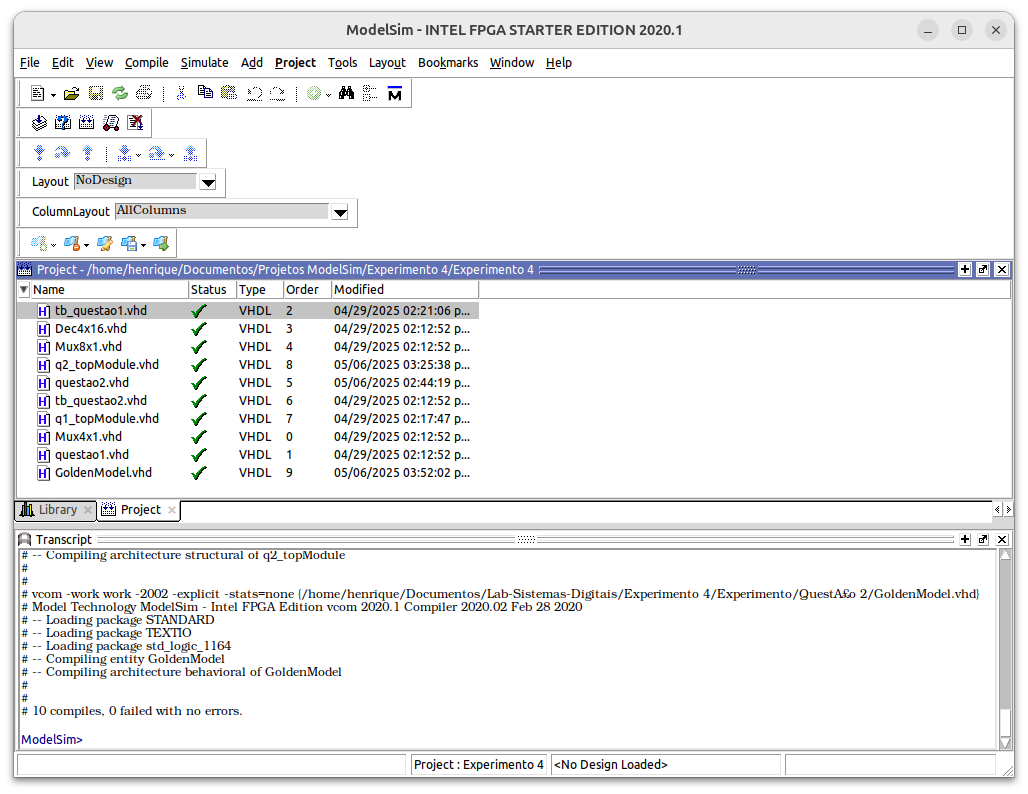
\includegraphics[width=0.8\textwidth]{Recursos/Imagens/CompileModelSim.png}
    \caption{Compilação de todos os códigos apresentados}
\end{figure}

\section{Simulação}
O gráfico de forma de onda gerado pelo ModelSim ao simular o \textit{top-module} está exibido abaixo. Foram marcados com cursores os momentos de interesse para a análise.

\begin{figure}[H]
    \centering
    \begin{tcolorbox}[colframe=cinza, colback=white, boxrule=0.75pt, arc=0pt, width=1\textwidth, center, boxsep=0pt, left=0pt, right=0pt, top=0pt, bottom=0pt]
    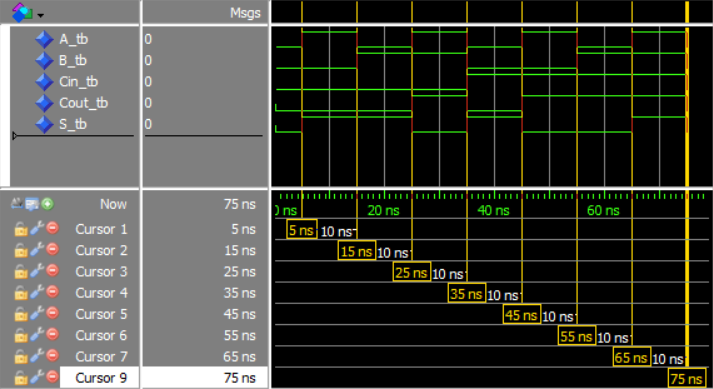
\includegraphics[width=1\textwidth]{Recursos/Imagens/waves.png}
    \end{tcolorbox}
    \caption{Simulação em forma de onda binária do registrador}
    \label{fig: ondas}
\end{figure}

\section{Análise}
Na onda apresentada na \autoref{fig: ondas}, estão marcados os momentos cruciais do teste. Esses instantes são: 
\begin{enumerate}
    \item 4 ns - \textit{reset} assíncrono;
    \item 20 ns - tentativa de \textit{load} (não ocorre pois o \textit{reset} segue em 1);
    \item 40 ns - \textit{load};
    \item 60 ns - \textit{shift left} (entra o 0 na direita);
    \item 80 ns - \textit{shift right} (entra o 0 na esquerda).
\end{enumerate}
Analisando a saída $Q$, percebe-se que todas as instruções funcionam de acordo com o esperado. Podemos concluir, portanto, que a implementação apresentada está correta.

\section{Conclusão}
Neste experimento, tivemos o primeiro contato com flip-flops e, portanto, com circuitos sequenciais. Esses dispositivos são cruciais no projeto de máquinas de estados, além de serem base para o desenvolvimento de dispositivos mais complexos, como registradores, contadores, microprocessadores, etc.

Além disso, instanciando os flip-flops JK, desenvolvemos um registrador de deslocamento de 4 bits, dispositivo que é usado em máquinas de estados mais complexas e é essencial para a arquitetura de processadores digitais.

Em suma, chegamos a uma etapa essencial do estudo de sistemas digitais: começamos a entender o funcionamento em baixo nível dos dispositivos que se tornaram base para o desenvolvimento do mundo digital. É com base nisso que foram desenvolvidos os processadores digitais e, posteriormente, as linguagens de programação, sistemas operacionais, etc.
\end{document}